\documentclass[12pt]{report}

\usepackage[default]{sourcesanspro}
\usepackage[T1]{fontenc}
\usepackage{titlesec}
\usepackage{xcolor}
\usepackage{graphicx}
\usepackage{fancyhdr}
\usepackage{everypage}
\usepackage{soul} % For letter spacing and background color
\usepackage[letterspace=300]{microtype} 
\usepackage{background}
\usepackage[skip=10pt plus1pt]{parskip}
\usepackage{amsmath}
\usepackage[export]{adjustbox}

\usepackage[margin=2cm]{geometry}
\usepackage[ngerman]{babel}
\usepackage{tocloft}


\backgroundsetup{
  scale=1,
  color=white,
  opacity=0,
  angle=0,
  position=current page.center,
  vshift=0cm,
  hshift=0cm,
  contents={}
}

\definecolor{customlightblue}{HTML}{84B9D1} % Wortmaschinen
\definecolor{customlightpurple}{HTML}{8079B1} %Funktionsmaschinen 1
\definecolor{customred}{HTML}{C7857E} %Funktionsmaschinen 2
\definecolor{customyellow}{HTML}{D5B491} %Funktionen hören
\definecolor{customblue}{HTML}{8FA0D4} %Eigene Aufgaben
\definecolor{customgreen}{HTML}{89B19B} %Anleitung
\definecolor{bgblue}{HTML}{252944} %bgblue





\DeclareRobustCommand{\ebseries}{\fontseries{eb}\selectfont}
\DeclareTextFontCommand{\texteb}{\ebseries}

\DeclareRobustCommand{\sbseries}{\fontseries{sb}\selectfont}
\DeclareTextFontCommand{\textsb}{\sbseries}

\DeclareRobustCommand{\elseries}{\fontseries{el}\selectfont}
\DeclareTextFontCommand{\textel}{\elseries}

\DeclareRobustCommand{\lseries}{\fontseries{l}\selectfont}
\DeclareTextFontCommand{\textl}{\lseries}

\renewcommand{\seriesdefault}{l} % Set default series to light

\setlength{\parindent}{0pt} % Remove paragraph indentation




\titleformat{\chapter}
  {\color{white}\sffamily\sbseries\fontsize{22}{26}\selectfont } % Format of the chapter title
    {\thechapter.} % Chapter number
    {10pt} % Space between chapter number and title
    {} % Format of the chapter title text

\titlespacing*{\chapter}{0pt}{-18pt}{8pt} % Adjust the spacing
% Definition des ersten Hintergrunds
\newcommand{\backgroundOne}[1]{
  \backgroundsetup{
    scale=1,
    color=#1,
    opacity=1,
    angle=0,
    position=current page.north,
    vshift=-.8cm,
    hshift=-1cm,
    contents={\begin{tikzpicture}[remember picture,overlay]
      \fill[color=#1](current page.south west) rectangle (current page.north east);
    \end{tikzpicture}
    
\includegraphics[width=4.31cm, left]{../images/MATH-NODES_Logo.png}}   
  }
}

% Definition des zweiten Hintergrunds
\newcommand{\backgroundTwo}[1]{
  \backgroundsetup{
    scale=1,
    color=blue,
    opacity=1,
    angle=0,
    position=current page.north,
    vshift=-.8cm,
    hshift=-1cm,
    contents={\begin{tikzpicture}[remember picture,overlay]
      \fill[color=#1] (current page.north west) rectangle ([yshift=-1.76cm]current page.north east);
    \end{tikzpicture}
    
\includegraphics[width=4.31cm, left]{../images/MATH-NODES_Logo.png}}
  }
}

\renewcommand{\thesection}{\arabic{section}} 
\renewcommand{\thesubsection}{\arabic{section} \alph{subsection})}

\titleformat{\section}
  {\color{black}\sffamily\sbseries\fontsize{13}{30}\selectfont } % Format of the section title. Schriftgroeße 16. Zielenabstand 20
  {Aufgabe \thesection} % Section number
  {10pt} % Space between section number and title
  {} % Format of the section title text
  [\titlerule] % Add a black line under the section title

\titlespacing*{\section}{0pt}{12pt}{6pt} % Adjust the spacing

\titleformat{\subsection}
  {\color{black}\sffamily\sbseries\fontsize{12}{11}\selectfont } % Format of the subsection title
  {\thesubsection} % Subsection number
  {10pt} % Space between subsection number and title
  {} % Format of the subsection title text

  \titleformat{\subsubsection}
  {\color{black}\sffamily\sbseries\fontsize{12}{11}\selectfont } % Format of the subsection title
  {\thesubsubsection} % Subsection number
  {10pt} % Space between subsection number and title
  {} % Format of the subsection title text


\titlespacing*{\subsection}{0pt}{10pt}{5pt} % Adjust the spacing


% Defines TOC settings
%\setlength{\cftsecnumwidth}{5em} % Adjust the width of the section number
%\setlength{\cftsecindent}{2em} % Adjust the indent of the section title
%\setlength{\cftsubsecindent}{6em} % Adjust the indent of the subsection title
%\setlength{\cftsubsecnumwidth}{3em} % Adjust the width of the subsection number



% Define the chapter start page style with color
\newcommand{\chapterstartpage}[4]{
    \newpage % Start a new page
    \chapter{#1}
    % \addcontentsline{toc}{chapter}{#1} % Add the chapter title to the table of contents
    \backgroundOne{#3} % Erster Hintergrund
    \BgThispage % Hintergrund auf dieser Seite anwenden
    \color{white} % Set text color to white
    \vspace{-10pt}
   \rule{\textwidth}{0.8pt} % White line 0.8pt thick
    \newline\sffamily{\bfseries\fontsize{7}{9}\selectfont\textls[300]{#2}} % Subtitle in bold, size 7, all caps, letter spacing 30%
    \vspace{2cm}
   \newline \includegraphics[width=\textwidth]{#4}
  \newpage
  \color{black} % Set text color back to black
  \backgroundTwo{#3} % Zweiter Hintergrund
 % Hintergrund auf dieser Seite anwenden
% Entfernen des Hooks
}

\newcommand{\handwritinglines}[1]{
  \\[20pt]
  \noindent
  \foreach \i in {1,...,#1} {
    \rule{\textwidth}{0.25pt}\\[20pt]
  }
}



\begin{document}

\begin{titlepage}

    \backgroundsetup{
      scale=1,
      color=bgblue,
      opacity=1,
      angle=0,
      position=current page.center,
      vshift=0cm,
      hshift=0cm,
      contents={\begin{tikzpicture}[remember picture,overlay]
        \fill[color=bgblue] (current page.south west) rectangle (current page.north east);
      \end{tikzpicture}}
    }
    \BgThispage
    \color{white} % Set text color to white
    
\includegraphics[width=4.31cm, left]{../images/MATH-NODES_Logo.png}
    {\huge\bfseries Math-Nodes Arbeitsheft\par}

    \rule{\textwidth}{0.8pt} % White line 0.8pt thick
    %\vspace{8pt}
    \newline\sffamily{\bfseries\fontsize{7}{9}\selectfont\textls[300] {SPIELERISCH LERNEN MIT FUNKTIONSMASCHINEN\\
    EIN PROJEKT VON NICOLAS REGEL}} % Subtitle 
\vspace{3cm}\\
    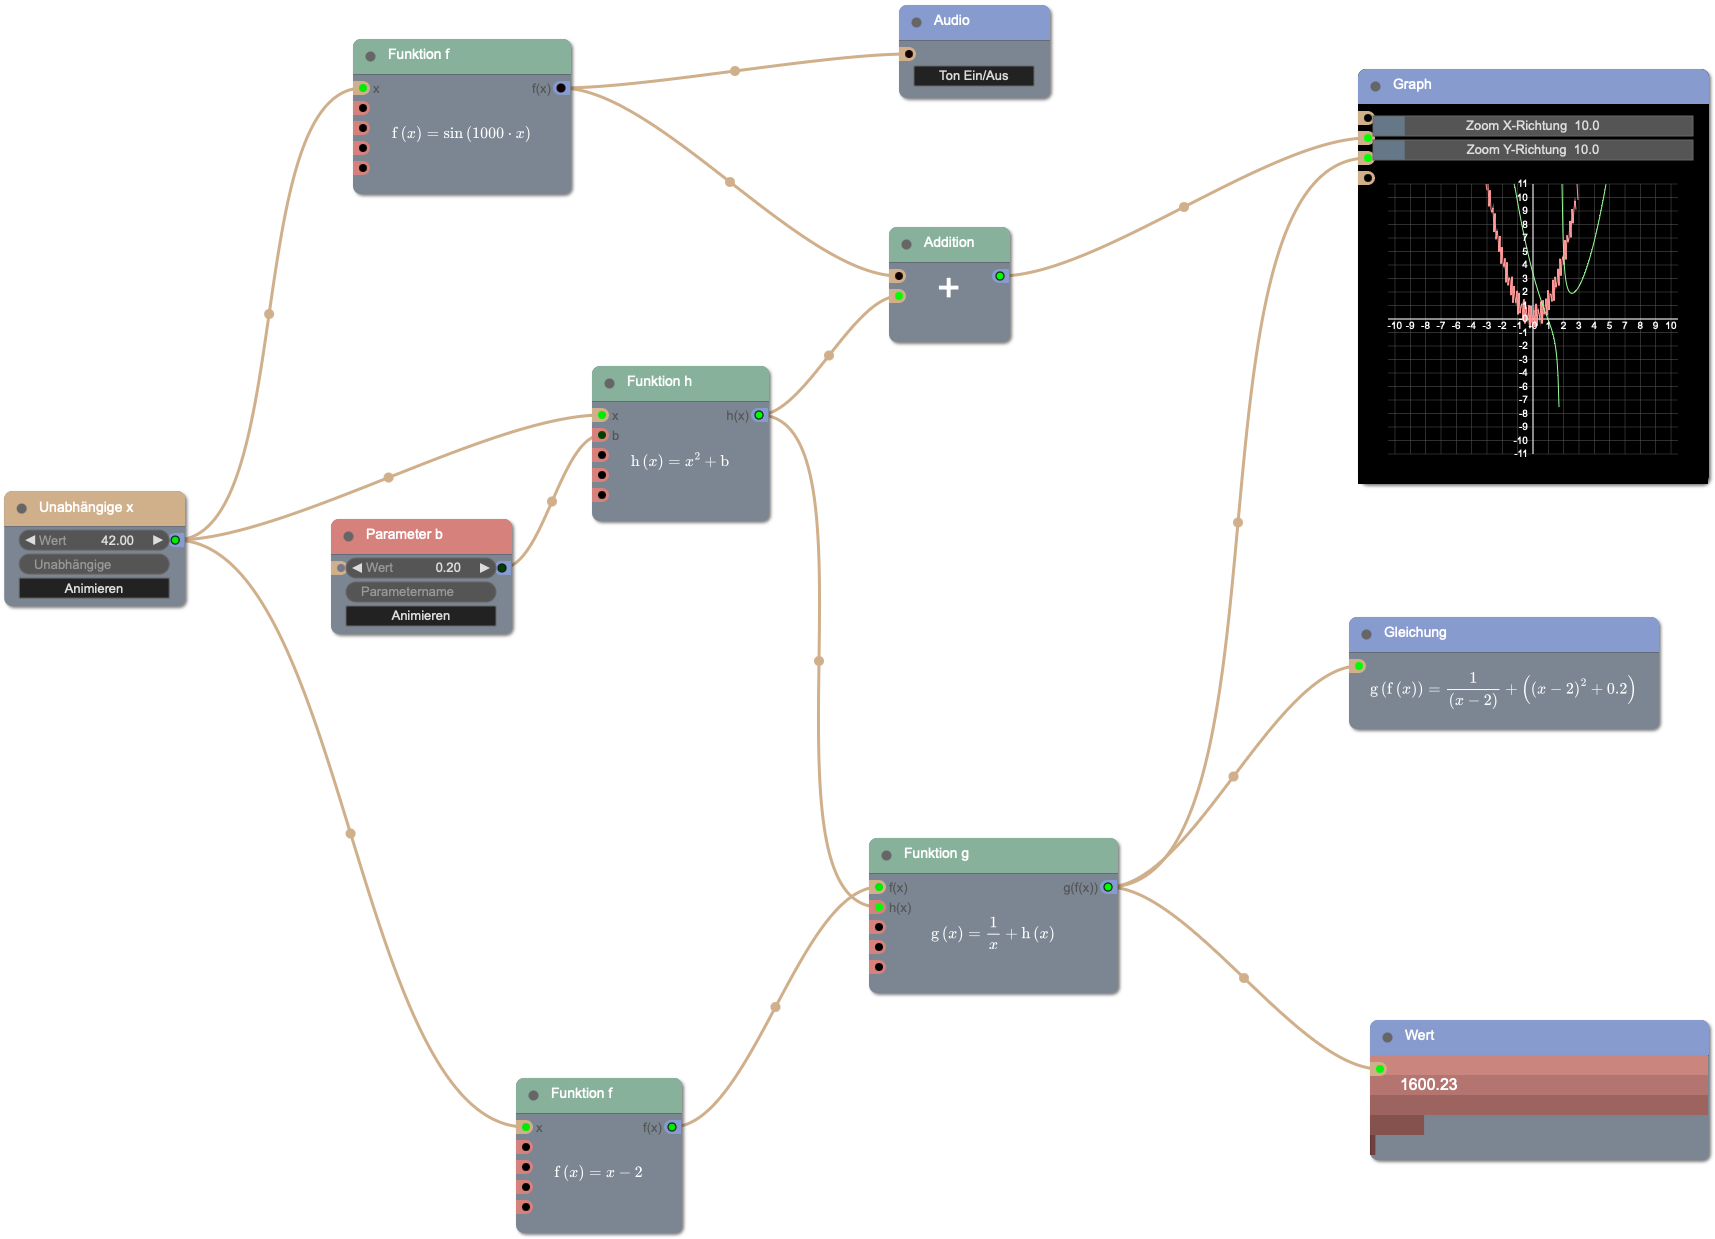
\includegraphics[width=\textwidth]{Bilder/Titel_Graph.png}
    \vspace{2.5cm}\\
    
\includegraphics[width=1.5cm, right]{../images/N_R_LOGO.png}

    \color{black} % Set text color to white
\end{titlepage}

\tableofcontents


% {\sffamily\elseries extra-light text}

% {\sffamily\lseries light text}

% {\sffamily regular text}

% {\sffamily\sbseries semi-bold text}

% {\sffamily\bfseries bold text}


\chapterstartpage{Wortmaschinen}{NACHRICHTEN VER- UND ENTSCHLÜSSELN}{customlightblue}{Bilder/Wortmaschinen_Titel.png}

\section{Deinen ersten Text verschlüsseln}
Du kannst deinen Text mit verschiedenen Maschinen manipulieren. Verbinde dazu die Texteingabe-Maschine mit der Vokaltanz-Maschine und diese dann mit der Text-Anzeige-Maschine. Was passiert mit deinem Text?
\par
Du kannst natürlich auch mehrere Maschinen hintereinander verwenden. Das nennt man in der Mathematik verketten. Die Maschinen bilden dann gemeinsam eine neue Maschine, die deinen Text in der verbundenen Reihenfolge verändert. Probiere es in MATH-NODES aus! Notiere in der Text Anzeige deine Ergebnisse:\par
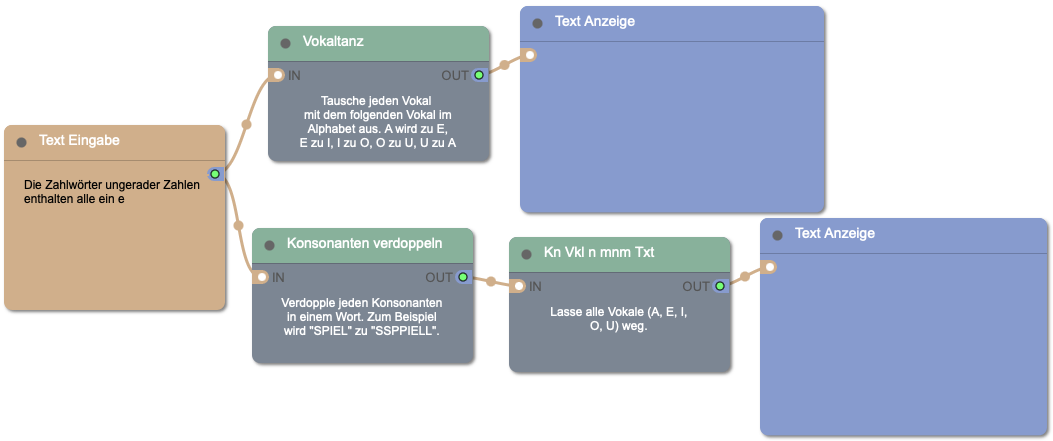
\includegraphics[width=\textwidth]{Bilder/Wortmaschinen_A1_config.png}

\section{ Maschinen verketten}
Zwei Maschinen kannst du in unterschiedlicher Reihenfolge verbinden. Spielt die Reihenfolge eine Rolle für das Ergebnis? Probiere es aus und begründe deine Antwort.\par
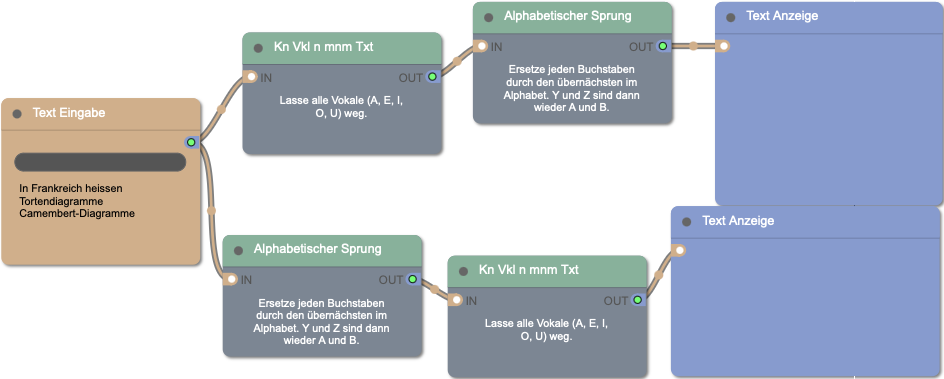
\includegraphics[width=\textwidth]{Bilder/Wortmaschinen_A2_config.png}
\handwritinglines{3}\\
Ist das immer so? Findest du zwei, bei denen die Reihenfolge egal ist? Gib die gefundenen Maschinen an, notiere den Ergebnis-Text und erkläre, was hier anders ist. Eine Übersicht über alle Wortmaschinen findest du am Ende dieses Arbeitsmaterials.\par
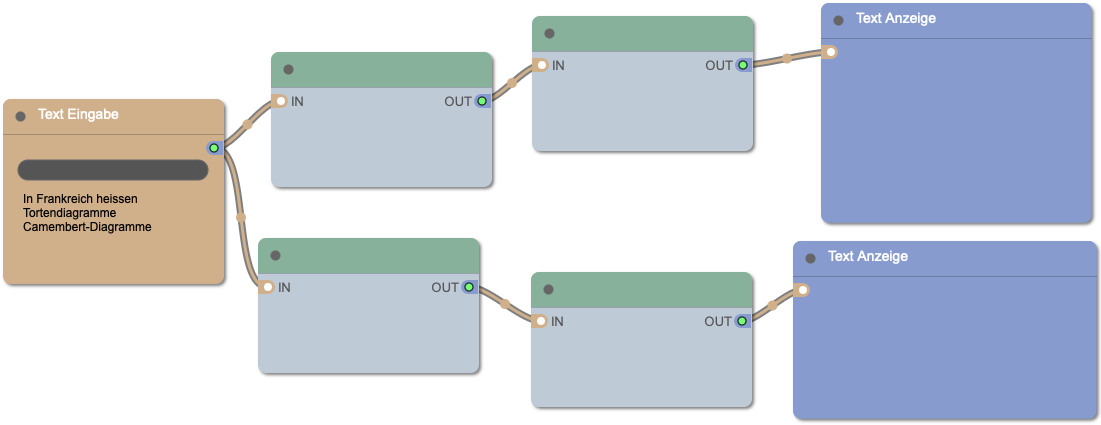
\includegraphics[width=\textwidth]{Bilder/Wortmaschinen_A2b_config.png}

\section{Welche Maschine war es?}
Hier sind zwei Nachrichten verschlüsselt worden. Einmal mit einer Maschine und einmal mit zwei Maschinen hintereinander.\par
Überlege erst was am Text verändert wurde und welche Maschinen es gewesen sein könnten. Probiere es aus und schreib den Namen der richtigen Maschine in das entsprechende Feld.\par
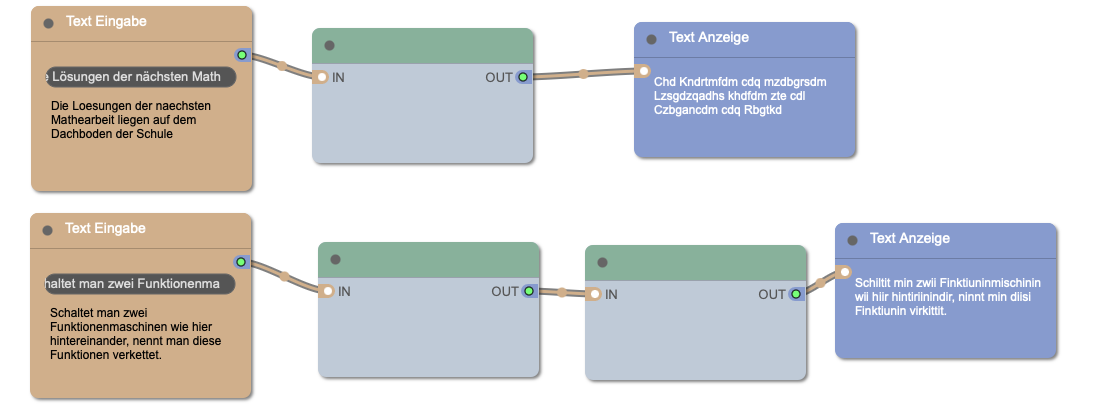
\includegraphics[width=\textwidth]{Bilder/Wortmaschinen_A3_config.png}


\section{Entschlüsseln einer Nachricht}
Mit der Alphabet-Countdown-Maschine wurde eine Nachricht verschlüsselt. Entwickle eine Maschine, um die Nachricht wieder zu entschlüsseln. Gib ihr einen Namen und beschreibe ihre Funktionsweise auf der Karte.\par
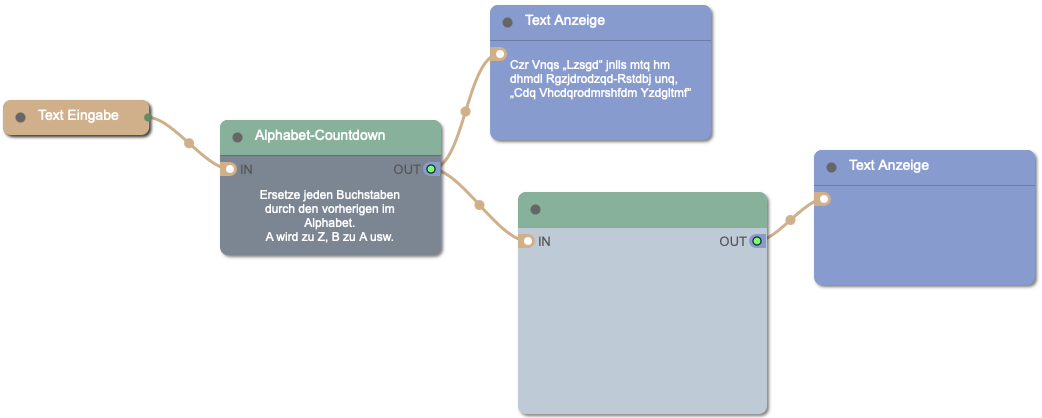
\includegraphics[width=\textwidth]{Bilder/Wortmaschinen_A4_config.png}\\
Genau die richtige Maschine zum Entschlüsseln der Botschaft scheint es in MATH-NODES nicht zu geben. Kannst du Sie aus anderen Maschinen zusammenbauen? Wie lautet die Botschaft? \\
\handwritinglines{2}

\section{ Umkehrbar oder nicht?}
Kannst du dir zu jeder Maschine eine Maschine ausdenken, die die damit verschlüsselte Nachricht wieder entschlüsselt?\par
Finde in MATH-NODES mindestens ein Beispiel, bei dem es nicht geht und begründe warum.\\
\handwritinglines{4}
\subsection{Bonusaufgabe:}
Mit welcher Maschine wurde hier verschlüsselt und wie kannst du das Rückgängig machen?\par
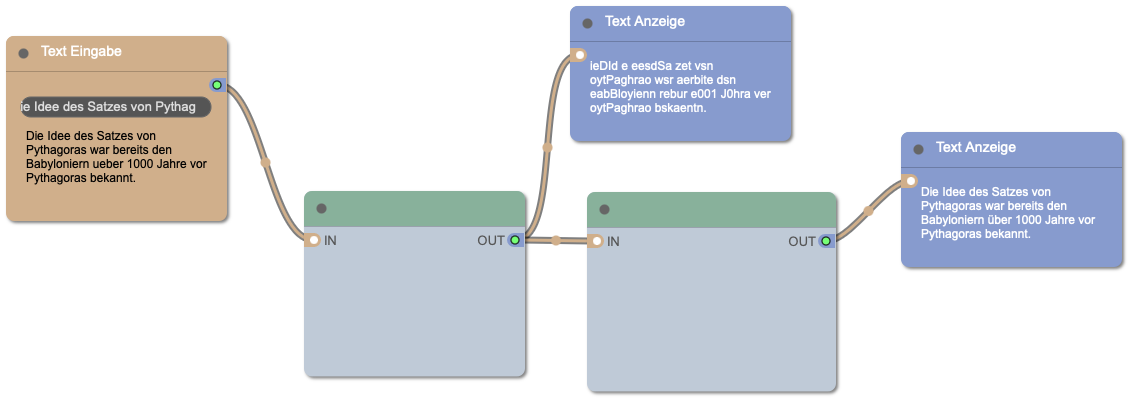
\includegraphics[width=\textwidth]{Bilder/Wortmaschinen_A5_config.png}
\handwritinglines{2}
\section{Umkehrfunktionen}
Überlege welche der Wortmaschinen Umkehrfunktionen zueinander sind. Gib Sie an, begründe deine Entscheidung und prüfe an einem Beispiel. Eine Übersicht über alle Maschinen findest du am Ende des Kapitels.\par
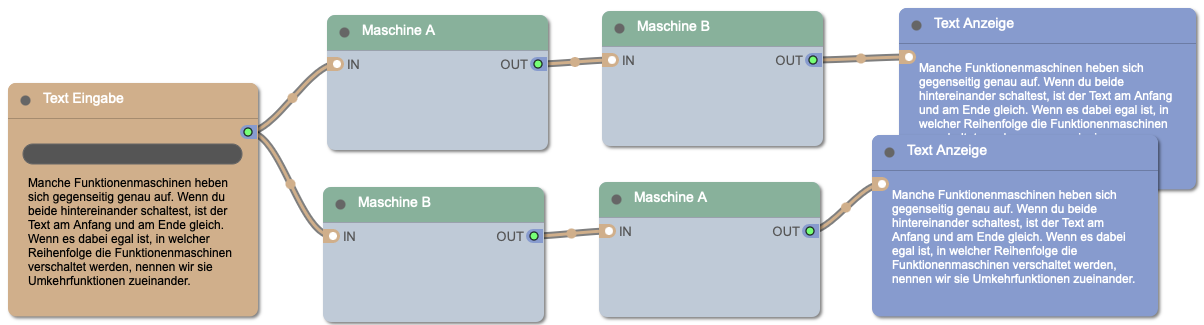
\includegraphics[width=\textwidth]{Bilder/Wortmaschinen_A6_config.png}
\handwritinglines{7}
\section{Geheime Nachrichten senden}
Überleg dir eine Nachrichten für die Person neben dir und schreib sie auf. Wähle bis zu drei Wortmaschinen zum Verschlüsseln aus, gib sie an und verschlüssele deine Nachricht damit. Achte bei der Auswahl deiner Wortmaschinen darauf, dass die Nachricht auch wieder entschlüsselbar ist.\par
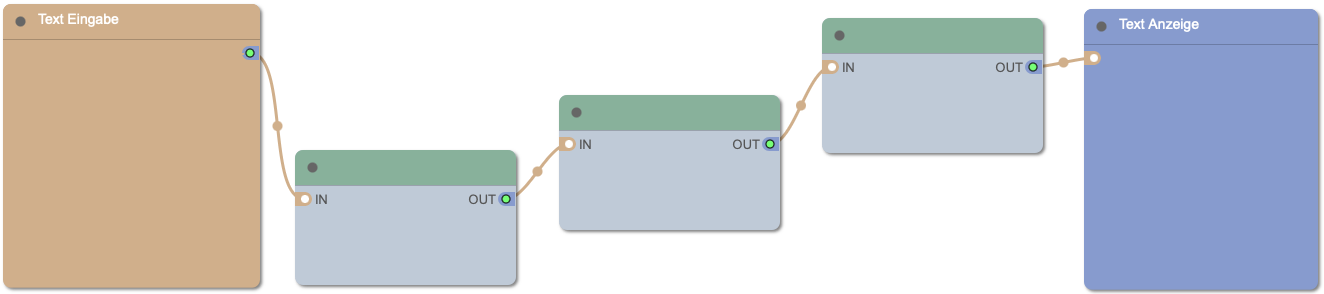
\includegraphics[width=\textwidth]{Bilder/Wortmaschinen_A7_config.png} 
\section{Geheime Nachrichten empfangen}
Tauscht eure verschlüsselten Nachrichten aus und probiert sie wieder zu entschlüsseln. Notiere deine empfangene Nachricht und deine Lösung.\par
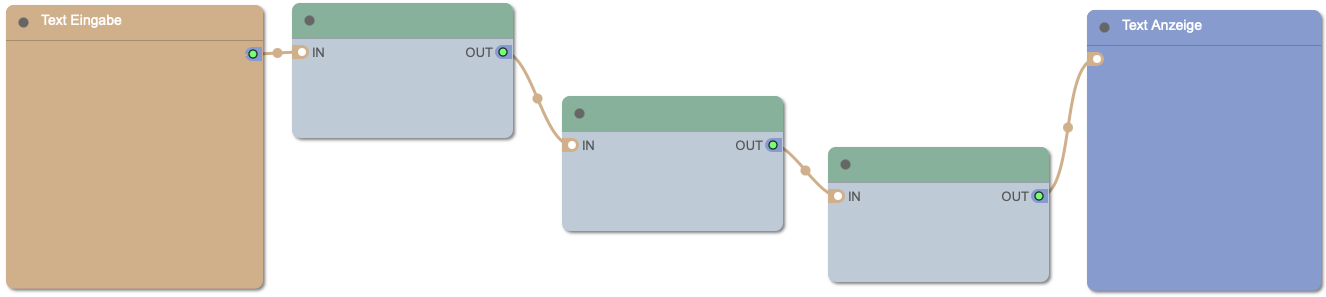
\includegraphics[width=\textwidth]{Bilder/Wortmaschinen_A8_config.png} 
\section*{Übersicht über alle Wortmaschinen}
\addcontentsline{toc}{section}{Übersicht über alle Wortmaschinen} % Add the chapter title to the table of contents 
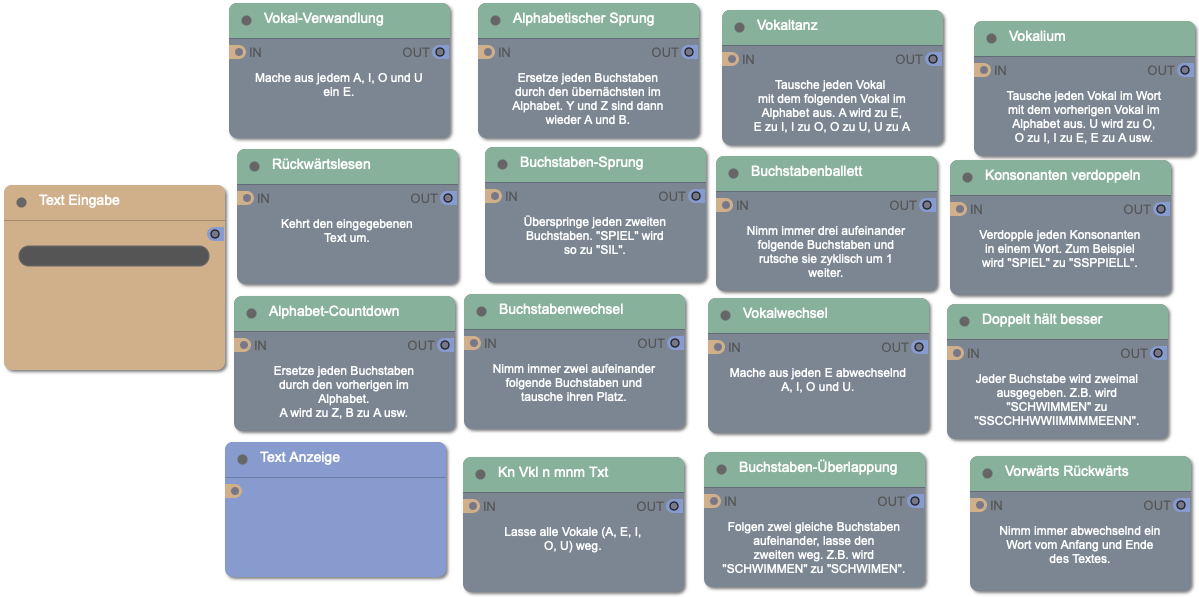
\includegraphics[width=\textwidth]{Bilder/Uebersicht_Wortmaschinen.png}
\chapterstartpage{Funktionsmaschinen}{MATHEMATISCHE FUNKTIONEN VERKNÜPFEN UND VERKETTEN LERNEN}{customlightpurple}{Bilder/Titel_Graph.png}
\section*{Funktionen als Maschinen}
Eine mathematische Funktion kannst du dir vorstellen wie eine Maschine mit einem Eingang und einem Ausgang. Man gibt etwas in die Maschine hinein und erhält dann etwas am Ausgang der Maschine. Eine wichtige Eigenschaft von Funktionen ist dabei, dass immer das Gleiche am Ausgang rauskommt, wenn wir das Gleiche am Eingang einwerfen. Auf dieser Seite lernst du damit umzugehen.
\section{Von der Wortmaschine zur Funktion}
Funktionsmaschinen funktionieren auf die gleiche Weise wie die Wortmaschinen. Genau genommen sind die Wortmaschinen auch spezielle Funktionsmaschinen.\par
Auch hier gibt es eine Eingabe in Form einer Maschine für die Unabhängige Variable. Diese wird von einer oder mehreren Funktionsmaschinen verarbeitet und das Ergebnis mit Hilfe von verschiedenen Feedback-Maschinen angezeigt.\par
Probiere verschiedene Werte aus und beobachte, wie sich das Ergebnis verändert.
\section{Funktionsmaschinen verketten}
Genau wie bei den Wortmaschinen kannst du auch Funktionsmaschinen hintereinander schalten. Die Maschinen bilden dann gemeinsam eine neue Maschine, die deinen Text in der verbundenen Reihenfolge verändert. Probiere verschiedene Kombinationen aus und notiere sie mit den Ergebnissen für die unabhängige Variable  im Arbeitsheft.
\subsection{Bonusaufgabe:}
Wie viele verschiedene Maschinen kannst du aus den 3 Funktionen bauen?

\section{Ergebnisse anders darstellen}
In Math-Nodes kannst du dir außer dem Wert zu einer unabhängigen Variable auch die Gleichung, den Graph und sogar den Ton einer Funktion ausgeben lassen. Dazu gibt es jeweils eine eigene Feedback-Maschine. Feedback-Maschinen sind immer blau. \par
Verbinde die Funktionen mit den verschiedenen Feedback-Maschinen und gib die Gleichung und den Graphen der verketteten Funktionen an. 
\section{Funktionsgleichungen ablesen}
Gib die Funktionsgleichung für die verketteten Funktionenmaschinen an
an. Skizziere den Graph. Überprüfe deine Ergebnisse in Math-Nodes.
\section{Funktionen verknüpfen}
Du kannst zwei Funktionsmaschinen nicht nur verketten, sondern auch mittels einer Operationsmaschine mit den typischen Operationen wie Addition, Multiplikation, usw. verknüpfen. Das siehst du hier im Beispiel.\par
Gib für die zweite Verknüpfung den Funktionsterm für die verknüpften Funktionenmaschinen an. Wie könnte der Graph aussehen? Diskutiere mit der Person neben dir. Skizziere den Graph.
\section{Verknüpfen und Verketten}
Verknüpfe und verkette die Maschinen so, dass du den angegebenen Funktionsterm erhältst. Wie könnte der Graph aussehen? Diskutiere mit der Person neben dir. Skizziere den Graph.
\section{Den Graphen treffen}
Verknüpfe und verkette die
Maschinen so, dass der grüne
Graph entsteht. Gib den
zugehörigen Funktionsterm an.
\section{Funktionenpuzzle}
Verknüpfe und/oder verkette die Maschinen so, dass die weißen Graphen entstehen. Gib jeweils den zugehörigen Funktionsterm an. Du brauchst nicht ganz alle Maschinen.

% Titelformate für Anleitung anpassen
  \renewcommand{\thesection}{\arabic{section}}
  \renewcommand{\thesubsection}{\arabic{section}.\arabic{subsection}}
  \renewcommand{\thesubsubsection}{\arabic{section}.\arabic{subsection}.\arabic{subsubsection}}

  \titleformat{\section}
  {\color{black}\sffamily\sbseries\fontsize{13}{30}\selectfont } % Format of the section title. Schriftgroeße 16. Zielenabstand 20
  {\thesection} % Section number
  {10pt} % Space between section number and title
  {} % Format of the section title text
  [\titlerule] % Add a black line under the section title
  

\chapterstartpage{Anleitung}{HIER FINDEST DU EINE DETAILLIERTE ANLEITUNG ZU ALLEN FUNKTIONEN VON MATH-NODES
}{customgreen}{Bilder/Wortmaschinen_Titel.png}
\section{Die Arbeitsoberfläche}
Die Arbeitsoberfläche von Math Nodes bietet eine intuitive und interaktive Umgebung zur Arbeit mit mathematischen Maschinen den MATH-NODES. Hier sind die grundlegenden Funktionen und Interaktionen, die auf der Arbeitsoberfläche möglich sind:
\subsection{Maschinen verschieben}
Maschinen können mit der Maus oder dem Finger frei in der Arbeitsfläche verschoben werden.
\subsection{Maschinen verbinden}
In MATH-NODES haben Maschinen Ein- und Ausgänge, die es ermöglichen, sie mit anderen Maschinen zu verbinden. Dazu benutzt du Kabel. An jedem Eingang darf nur ein Kabel angeschlossen werden, während an einem Ausgang beliebig viele Kabel angeschlossen werden können. Ausgänge sind blau und Eingänge orange markiert. Das Verbinden ist von beiden Seiten möglich. Wenn bereits ein Kabel vorhanden ist, kannst du es lösen, indem du es am Ende anfasst, oder ein neues Kabel erstellen, indem du es am Anfang anfasst.
\subsection{Maschinen hinzufügen}
Um eine neue Maschine hinzuzufügen, doppelklicke auf eine leere Stelle in der Arbeitsfläche oder auf eine bestehende Maschine, um sie zu ersetzen. Dadurch öffnet sich ein Menü, in dem du die gewünschte Maschinenart auswählen kannst. Alternativ kannst du das Menü auch über den Button "Neue Maschine" öffnen. Eine Maschine entfernen kannst du über die Zurücktaste deiner Tastatur oder das Menü.
\subsection{Zwischenwerte am Kabel ablesen}
In der Mitte jeder Kabelverbindung in Math-Nodes gib es einen kleinen Kreis. Wenn du die Maus darauf bewegst, wird dir das Zwischenergebnis angezeigt. Das ist oft schneller als eine extra Feedbackmaschine dort anzuschließen. Arbeitest du mit Wortmaschinen, wird dir dort der aktuelle Text angezeigt. Bei den Funktionsmaschinen der aktuelle Wert abhängig vom eingestellten Wert der unabhängigen Variablen. 
\subsection{Leuchten an den Ein- und Ausgängen}
Bestimmt ist dir schon aufgefallen, dass die Ein- und Ausgänge der einzelnen Maschinen verschiedenfarbig leuchten. Helligkeit und Farbe sind dabei nicht zufällig, sondern geben visuelles Feedback über die Werte, die durch die Verbindungen fließen. Positive Werte werden in verschiedenen Grüntönen dargestellt -je heller desto größer der Wert- , während negative Werte in verschiedenen Rottönen angezeigt werden -je heller, desto kleiner der Wert-. Die Farben können natürlich nicht unendlich hell werden, sodass der Helligkeitsunterschied immer kleiner wird, je größer bzw. kleiner der Wert wird.
\subsection{Einstellungen von Maschinen ändern}
Mansche Maschinen haben Textfelder oder Knöpfe, sodass du Einstellungen und Werte der Maschine verändern kannst. Zum Ändern der entsprechenden Einstellungen musst du einfach in das Textfeld oder auf den Button klicken. Durch Drücken und Ziehen kannst du Schieberegler wie z.B. bei den Feedback Maschine für den Graphen bearbeiten. 
\subsection{Maschinen einklappen}
Wenn du den Überblick verlierst, kannst du Maschinen einklappen. Dazu klickst du auf den Kreis oben links in der Maschine. Genauso kannst du sie wieder ausklappen. In manchen Aufgaben findest du Maschinen, die schon eingeklappt sind und sich nicht ausklappen lassen. Das ist Absicht, um dir die Lösung einer Aufgabe nicht zu verraten.

\subsection{Das Menü}
Jeder Arbeitsfläche bei Math-Nodes hat ein eigenes Menü, das verschiedene Funktionen bereitstellt. Das sind die wichtigsten Funktionen: Vollbild, Als Bild speichern, Speichern, Laden, Alles Löschen, Neue Maschine, Zoom, Maschinen sortieren, Maschine löschen.
\subsubsection{Vollbild}
Schaltet die Ansicht in den Vollbildmodus, sodass du mehr Platz hast, um mit deinen Maschinen zu arbeiten. Um den Vollbildmodus zu verlassen, drücke die Esc-Taste oder klicke erneut auf die Vollbild-Schaltfläche.

\subsubsection{Als Bild speichern}
Speichert die aktuelle Ansicht der Arbeitsfläche als Bilddatei. Dies ist nützlich, um deine Arbeit zu dokumentieren oder zu teilen.
\subsubsection{Speichern}
Speichert den aktuellen Zustand der Arbeitsfläche, damit du später weiterarbeiten kannst. Du kannst deine Arbeit jederzeit laden und fortsetzen. Die Datei wird lokal auf deinem Computer gespeichert und kann in jede Arbeitsfläche auf Math-Nodes geladen werden.
\subsubsection{Laden}
Lädt einen zuvor gespeicherten Zustand der Arbeitsfläche. Dies ermöglicht es dir, an einem früheren Punkt deiner Arbeit weiterzumachen. So kannst du z.B. auch eigene Aufgaben erstellen. Unter (hier noch nicht bestehende Seite verlinken) gibt es eine leere Arbeitsoberfläche, die dafür gedacht ist.
\subsubsection{Alles Löschen}
Entfernt alle Maschinen von der Arbeitsfläche. Du wirst nochmal gewarnt, ob du das wirklich möchtest.
\subsubsection{Neue Maschine}
Öffnet ein Menü, in dem du neue Maschinen auswählen und zur Arbeitsfläche hinzufügen kannst. Du kannst zwischen verschiedenen Maschinenarten wählen. Je nachdem, wo auf Math-Nodes du dich befindest, stehen dir die Wort- oder die Funktionsmaschinen zur Verfügung. Eine leere Arbeitsfläche, wo du beides verwenden kannst, findest du auf (Seite noch erstellen). In dieses Menü kommst du auch, wenn du doppelt auf eine leere Stelle im Arbeitsfenster klickst oder doppelt auf eine Maschine. Im letzteren Fall wird die geklickte Maschine durch die neue ersetzt. Das ist nützlich, wenn du z.B. verschiedene Wortmaschinen ausprobieren willst. Du verlässt das Menü über den Knopf oben rechts. Wenn du über den Doppelklick in das Menü gekommen bist, schließt es sich auch nach Auswahl einer neuen Maschine automatisch.
\subsubsection{Zoom}
Vergrößert oder verkleinert die Ansicht der Arbeitsfläche. Das brauchst du z.B., wenn du ein kleines Display hast.
\subsubsection{Maschinen sortieren}
Die Maschinen werden automatisch auf der Arbeitsfläche positioniert, um eine optimale Übersicht zu gewährleisten. Dabei werden die Abstände zwischen den Maschinen maximiert, die Positionen der Maschinen untereinander aber möglichst beibehalten. Wenn du die Fenstergröße änderst oder in oder aus dem Vollbildmodus wechselst, passiert das automatisch. Du kannst die Funktion auch nutzen, wenn du aus Versehen eine Maschine aus dem Arbeitsfenster geschoben hast.
\subsubsection{Maschine löschen}
Entfernt die ausgewählte Maschine von der Arbeitsfläche. Dies ist nützlich, wenn du eine Maschine nicht mehr benötigst.
\section{Wortmaschinen}
Die Wortmaschinen sind in Math-Nodes ein einfacher Einstieg in die Welt der mathematischen Funktionen. Grundlegende Konzepte des Funktionsbegriffs wie Eindeutigkeit, Verkettung, Umkehrbarkeit können hier spielerisch erlernt werden, bevor sie dann mit den Funktionsmaschinen vertieft werden. 
\subsection{Wortmaschinen verketten}
Du kannst natürlich auch mehrere Maschinen hintereinander verwenden. Es werden dann einfach alle Manipulationen des Textes nacheinander ausgeführt. Du kannst zwischenergebnisse an den Kreisen in der Mitte der Kabel prüfen oder indem du eine Text-Anzeige-Maschine dazwischen schaltest.
\subsection{Einzelne Maschinen im Detail}
Hier ist die Funktion aller Wortmaschinen einzeln aufgeführt. Generell für alle gilt, dass nur die Buchstaben A-Z bzw. a-z verändert werden. Sonder- und Leerzeichen bleiben unverändert.
\subsubsection{Text Eingabe}
Mit der Text Eingabe Maschine kannst du Text eingeben, der dann von anderen Maschinen weiterverarbeitet wird. Beispiel: "Hallo Welt".

\subsubsection{Text Anzeige}
Die Text Anzeige Maschine zeigt den Text an, der von anderen Maschinen verarbeitet wurde. Beispiel: "Hallo Welt" wird angezeigt.

\subsubsection{Alphabet-Countdown}
Ersetzt jeden Buchstaben durch den vorherigen im Alphabet. Beispiel: "BCD" wird zu "ABC".

\subsubsection{Rückwärtslesen}
Kehrt den eingegebenen Text um. Beispiel: "Hallo" wird zu "ollaH".

\subsubsection{Vokal-Verwandlung}
Ersetzt alle Vokale (A, I, O, U) durch E. Beispiel: "Hallo" wird zu "Helle".

\subsubsection{Kn Vkl n mnm Txt}
Lässt alle Vokale (A, E, I, O, U) weg. Beispiel: "Hallo Welt" wird zu "Hll Wlt".

\subsubsection{Buchstabenwechsel}
Tauscht immer zwei aufeinanderfolgende Buchstaben. Beispiel: "Hallo" wird zu "aHlol".

\subsubsection{Buchstaben-Sprung}
Überspringt jeden zweiten Buchstaben. Beispiel: "SPIEL" wird zu "SIL".

\subsubsection{Alphabetischer Sprung}
Ersetzt jeden Buchstaben durch den übernächsten im Alphabet. Beispiel: "ABC" wird zu "CDE".

\subsubsection{Buchstaben-Überlappung}
Lässt den zweiten Buchstaben weg, wenn zwei gleiche Buchstaben aufeinander folgen. Beispiel: "SCHWIMMEN" wird zu "SCHWIMEN".

\subsubsection{Vokalwechsel}
Ersetzt jedes E abwechselnd durch A, I, O und U. Beispiel: "Essen" wird zu "Assin".

\subsubsection{Buchstabenballett}
Verschiebt immer drei aufeinanderfolgende Buchstaben zyklisch um 1 weiter. Beispiel: "ABCDEF" wird zu "BCDAEF".

\subsubsection{Vokaltanz}
Ersetzt jeden Vokal durch den folgenden Vokal im Alphabet. Beispiel: "Hallo" wird zu "Helle".

\subsubsection{Vokalium}
Ersetzt jeden Vokal durch den vorherigen Vokal im Alphabet. Beispiel: "Hallo" wird zu "Hillu".

\subsubsection{Konsonanten verdoppeln}
Verdoppelt jeden Konsonanten in einem Wort. Beispiel: "SPIEL" wird zu "SSPPIELL".

\subsubsection{Doppelt hält besser}
Jeder Buchstabe wird zweimal ausgegeben. Beispiel: "SCHWIMMEN" wird zu "SSCCHHWWIIMMMMEENN".

\subsubsection{Vorwärts Rückwärts}
Nimmt immer abwechselnd ein Wort vom Anfang und Ende des Textes. Beispiel: "Eins Zwei Drei Vier" wird zu "Eins Vier Zwei Drei".

\section{Funktionsmaschinen}
Eine mathematische Funktion kannst du dir vorstellen wie eine Maschine mit einem Eingang und einem Ausgang. Man gibt etwas in die Maschine hinein und erhält dann etwas am Ausgang der Maschine. Eine wichtige Eigenschaft von Funktionen ist dabei, dass immer das Gleiche am Ausgang rauskommt, wenn wir das Gleiche am Eingang einwerfen. Um Funktionsmaschinen in Math-Nodes zu verwenden brauchst du also mindestens 3 Dinge. Eine unabhängige Variable, also das, was du in die Funktionsmaschine hinein gibts und eine Art dir das Ergebnis hinterher anzugucken. In Math-Nodes sind die unabhängige Variable und das Feedback, also das, was du dir von der Funktion anschaust, selbst durch kleine Maschinen repräsentiert. 
\subsection{Eine Funktionsmaschine verwenden}
In diesem einfachen Beispiel ist die unabhängige Variable mit der Funktion und der Wert-Feedback-Maschine verbunden. Du kannst dir so anschauen, welchen Funktionswert die Funktion für den jeweils eingestellten Wert der unabhängigen Variable annimmt. Du musst darauf achten, dass der Name der unabhängigen Variable mit der in deiner Funktion verwendeten übereinstimmt und du den ersten Eingang deiner Funktionsmaschine verwendest. 
\subsection{Feedbackmaschinen verwenden}
Wie schon angedeutet gibt es verschiedene Arten des Feedbacks in Math-Nodes. Du kannst dir deine Funktion also auf verschiedene Weise anschauen. Jede Feedbackart hat eine eigene Maschine. Du kannst Sie also jeweils einzeln, aber auch alle gleichzeitig anschließen. Feedbackmaschinen sind in Math-Nodes blau.
\subsubsection{Wert}
Die Wert Maschine zeigt den Wert der anhängigen Variable einer mathematischen Funktion an, also den Wert am Ausgang der Funktion und gibt zusätzlich grafisches Feedback. 
Beispiel: Wenn die Funktion $f(x) = x + 2$ ist und $x = 3$, dann zeigt die Maschine den Wert $5$ an. 
Das grafische Feedback zeigt den Wert als Anteil farbiger Balken an, wobei positive Werte in verschiedenen Rottönen und negative Werte in verschiedenen Blautönen dargestellt werden. Der Anteil an unterschiedlichen Wertebereichen wird bis $1.000.000$ untereinander und dann übereinander angezeigt. Die Wertebereiche sind $10$, $100$, $1000$, $10.000$, $100000$, $1.000.000$, $10.000.000$, $100.000.000$, $1.000.000.000$ und $10.000.000.000$.
\subsubsection{Gleichung}
Die Gleichung Maschine zeigt die mathematische Gleichung an, die als Eingabe verwendet wird. Beispiel: Wenn die Eingabe $f(x) = x + 2$ ist, dann zeigt die Maschine $f(x) = x + 2$ an. Wenn du Funktionen verkettest gibt sie die Gesamtgleichung aus, je nachdem wo sie angeschlossen ist.
\subsubsection{Graph}
Die Graph Maschine zeichnet den Graphen einer oder mehrerer mathematischer Funktionen. Beispiel: Wenn die Eingabe $f(x) = x + 2$ ist, dann zeigt die Maschine den Graphen dieser Funktion an.
\subsubsection{Audio}
Mit der Audio Maschine kannst du periodische Funktionen hörbar machen. Damit du auch wirklich was hörst, musst du darauf achten, dass sie eine Frequenz zwischen 60 Hz und 13.000 Hz haben. Welche Funktionen geeignet sind, lernst du im Workshop Funktionen hören  
Wichtig: Auch, wenn du den Ton an der Audio-Maschine anschaltest, wird er nur ausgegeben, wenn die Funktion „läuft“, du die Animation also an der Unabhängige Variable Maschine gestartet hast. Die Audiowiedergabe startet auch an dem Wert der unabhängigen Variable die in der zugehörigen Maschine eingestellt ist.
\subsection{Funktionen verketten}
\subsection{Funktionen verknüpfen}
\subsection{Parameter verwenden}
\subsection{Funktionen hören}
\subsection{Einzelne Maschinen im Detail}
\subsubsection{Unabhängige Variable}
Die Unabhängige-Variable-Maschine ist der Ausgangspunkt jeder Verkabelung mit den Funktionsmaschinen Math-Nodes. Sie ist das Etwas, das Objekt, das du in die Funktionsmaschinen hineingibst. Die Maschine hat folgende Funktionen:

\begin{itemize}
    \item \textsb{Wert einstellen:} Mit dem Zahlen-Widget kannst du den Wert der unabhängigen Variablen einstellen. In den einzelnen Funktionsmaschinen taucht er mit seinem Namen z.B. $x$ auf, in der Feedback-Maschine Wert siehst du dann aber das Ergebnis, also die abhängige Variable zu deinem hier eingestellten Wert.
    
    \item \textsb{Name der Variablen:} Im Text-Widget kannst du den Namen der unabhängigen Variablen frei wählen. Beachte, dass nur einzelne Buchstaben erlaubt sind und bestimmte Buchstaben wie 'e' und 'i' nicht verwendet werden können. Der hier verwendete Name muss mit den Namen der unabhängigen Variablen in den einzelnen Funktionsmaschinen übereinstimmen.
    
    \item \textsb{Animation:} Mit dem Button "Animation" kannst du die Animation der unabhängigen Variablen aktivieren oder deaktivieren. Wenn die Animation aktiviert ist, steigt der Wert der Variablen ausgehend von deinem eingestellten Startwert kontinuierlich an. So kannst du die Funktionen in Echtzeit verfolgen und z.B. das Wachstumsverhalten zweier Funktionen miteinander vergleichen. Außerdem startest du so auch die Tonausgabe, wenn du die Audio-Feedback-Maschine nutzt.
    
    \item \textsb{Titel:} Im Titel der Maschine siehst du immer den Namen der unabhängigen Variablen. Wenn die Animation aktiv ist, wird zusätzlich der aktuelle Wert angezeigt.
\end{itemize}

Diese Funktionen machen die UV-Maschine zu einem wichtigen Werkzeug, um mit unabhängigen Variablen in deinen Projekten zu arbeiten.
\subsubsection{Parameter}
Die Parameter-Maschine funktioniert ähnlich wie die Unabhängige-Variable-Maschine, nur, dass du Sie nur an den Parameter-Eingang der Funktionsmaschinen anschließen kannst. Der Eingestellte Wert wird dann in der Funktion direkt übernommen. Du kannst auch hier eine Animation starten, um dir z.B. in der Graph-Maschine anzuschauen, wie sich die Funktion bei der Veränderung des Parameters verhält.
\subsubsection{Funktion}
\subsubsection{Operation}
\subsubsection{Feedback Gleichung}
Die Gleichung Maschine zeigt die mathematische Gleichung an, die als Eingabe verwendet wird. Beispiel: Wenn die Eingabe $f(x) = x + 2$ ist, dann zeigt die Maschine $f(x) = x + 2$ an. Wenn du Funktionen verkettest gibt sie die Gesamtgleichung aus, je nachdem wo sie angeschlossen ist.
\subsubsection{Feedback Wert}
Die Wert Maschine zeigt den Wert der anhängigen Variable einer mathematischen Funktion an, also den Wert am Ausgang der Funktion und gibt zusätzlich grafisches Feedback. 
Beispiel: Wenn die Funktion $f(x) = x + 2$ ist und $x = 3$, dann zeigt die Maschine den Wert $5$ an. 
Das grafische Feedback zeigt den Wert als Anteil farbiger Balken an, wobei positive Werte in verschiedenen Rottönen und negative Werte in verschiedenen Blautönen dargestellt werden. Der Anteil an unterschiedlichen Wertebereichen wird bis $1.000.000$ untereinander und dann übereinander angezeigt. Die Wertebereiche sind $10$, $100$, $1000$, $10.000$, $100000$, $1.000.000$, $10.000.000$, $100.000.000$, $1.000.000.000$ und $10.000.000.000$.
\subsubsection{Feedback Graph}
Die Graph-Maschine kannst du nutzen, um die Graphen zu deinen Funktionen zu visualisieren:
\begin{itemize}
    \item \textsb{Eingänge für Funktionen}: Die Maschine hat vier Eingänge, an die verschiedene mathematische Funktionen angeschlossen werden können. Jede Funktion wird in einer anderen Farbe dargestellt.
    \item \textsb{Zoom-Funktion}: Es gibt zwei Schieberegler (Widgets) für die Zoom-Einstellungen in X- und Y-Richtung. Diese Regler ermöglichen es, den Wertebereich der X- und Y-Achsen anzupassen.
    \item \textsb{Gitternetzlinien}: Die Maschine zeichnet Gitternetzlinien, die sich an der Skalierung der Achsen orientieren. Diese Linien helfen, die Positionen der Punkte auf dem Graphen besser zu erkennen.
    \item \textsb{Achsenbeschriftungen}: Die X- und Y-Achsen sind mit Beschriftungen versehen, die die aktuellen Werte anzeigen. Diese Beschriftungen passen sich automatisch an den Zoom und die Skalierung an.
    \item \textsb{Farbige Darstellung}: Jede der vier Funktionen wird in einer eigenen Farbe dargestellt, um sie leicht unterscheiden zu können.
    \item \textsb{Diskontinuitäten erkennen}: Die Maschine erkennt Diskontinuitäten in den Funktionen und unterbricht die Linienzeichnung, um diese korrekt darzustellen.
    \item \textsb{Hintergrundfarbe}: Die Hintergrundfarbe des Graphen kann zwischen Schwarz und Weiß umgeschaltet werden.
    \item \textsb{Speichern von Gleichungen}: Es gibt die Möglichkeit, eine Gleichung und die zugehörigen Variablen zu speichern und später wieder abzurufen.
  \end{itemize}
Beachte, dass es bei sehr schnell oszillierenden Funktionen z.B. Sinusfunktionen mit einer Frequenz im hörbaren Bereich zu Darstellungsfehlern kommen kann. In diesem Fall solltest du die Frequenz der Funktion verringern.  
\subsubsection{Feedback Audio}
Mit der Audio Maschine kannst du periodische Funktionen hörbar machen. Damit du auch wirklich was hörst, musst du darauf achten, dass sie eine Frequenz zwischen $60\,Hz$ und $13.000\, Hz$ haben. Welche Funktionen geeignet sind, lernst du im Workshop Funktionen hören  
Wichtig: Auch, wenn du den Ton an der Audio-Maschine anschaltest, wird er nur ausgegeben, wenn die Funktion „läuft“, du die Animation also an der Unabhängige Variable Maschine gestartet hast. Die Audiowiedergabe startet auch an dem Wert der unabhängigen Variable die in der zugehörigen Maschine eingestellt ist.
\section{Infos für Expert:innen}
\subsection{Widgets verstecken}
\subsection{Graphen speichern}
\newpage
\begin{titlepage}

  \backgroundsetup{
    scale=1,
    color=bgblue,
    opacity=1,
    angle=0,
    position=current page.center,
    vshift=0cm,
    hshift=0cm,
    contents={\begin{tikzpicture}[remember picture,overlay]
      \fill[color=bgblue] (current page.south west) rectangle (current page.north east);
    \end{tikzpicture}}
  }
  \BgThispage
  \color{white} % Set text color to white
  
\includegraphics[width=4.31cm, left]{../images/MATH-NODES_Logo.png}
  
\includegraphics[width=1.5cm, right]{../images/N_R_LOGO.png}
  %{\huge\bfseries Math-Nodes Arbeitsheft\par}
  \vspace{19.5cm}\\
  \rule{\textwidth}{0.8pt} % White line 0.8pt thick
  %\vspace{8pt}
  \newline\sffamily{\bfseries\fontsize{7}{9}\selectfont\textls[300] {SPIELERISCH LERNEN MIT FUNKTIONSMASCHINEN\\
  EIN PROJEKT VON NICOLAS REGEL}} % Subtitle 
  
  \color{black} % Set text color to white
\end{titlepage}

\end{document}